\documentclass{article}
\usepackage{amssymb, amsmath, amsthm}
\usepackage[margin=1in]{geometry}
\usepackage{verbatim}
\usepackage{graphicx}
\usepackage{hyperref} % \url \href
\usepackage{docmute}

\newtheorem{definition}{Definition}
\newtheorem{theorem}{Theorem}
\newcommand{\heff}{\mathbb{H}^{\text{eff}}}
\newcommand{\pfrac}[2]{\frac{\partial #1}{\partial #2}}

\newcommand{\MO}{\textbf{MO}}
\newcommand{\AO}{\textbf{AO}}

\newcommand{\huptb}{\text{H}_0}
\newcommand{\order}[2]{#1^{(#2)}}
\newcommand{\statebra}[1]{\langle #1 |}
\newcommand{\stateket}[1]{| #1 \rangle}

\begin{document}

\section{Molecular Orbitals in Conjugated System and Solids}
\subsection{Conjugated System}
Conjugated system\footnote{\url{https://en.wikipedia.org/wiki/Conjugated_system}} 
refer to systems consists of connected $p$ orbitals with delocalized electrons in a molecular. 
Let's consider $N$ $\pi$ orbitals along a chain with nearest neighbor interaction and 
we further assume that their orbitals are non-overlapping so that the matrix 
element is $S_{\mu\nu} = \delta_{\mu\nu}$. 
The reason that we choose $\pi$ orbital system is because the small orbital overlap in this 
situation, as compared to the head to head sigma interactions. 
Let the energy of the $p$ orbital itself to be $\alpha$
and the nearest neighbor interaction $\beta < 0$, the secular equation can be reduced to 
an eigen-equation:
\begin{equation}
    H^{AO} \mathbf{C}_i = \varepsilon_i \mathbf{C}_i
\end{equation}
where the form of the Hamiltonian is like:
\begin{equation}
    H^{AO}_{N=3} = \left(\begin{matrix}
        \alpha & \beta & 0 \\ 
        \beta & \alpha & \beta \\ 
        0 & \beta & \alpha 
    \end{matrix}\right)
\end{equation}
The solution of the eigen-equation is given by:
\begin{align}
    \varepsilon_j &= \alpha + 2 \beta \cos\frac{j\pi}{N+1} \\ 
    c_{\mu j} &= \left(\frac{2}{N+1}\right)^{1/2} \sin\left(\frac{\mu j\pi}{N+1}\right) 
\end{align}
where $j$ index\footnote{$j$ is used instead of $i$ to avoid confusion with imaginary number $i$} 
the obtained molecular orbital and $\mu$ index the consistuting atomic orbitals. 

The importance of the factor $N+1$ can be shown as follows: we subsitute the solution into the 
eigen-equation:
\begin{equation}
    \sum_{\nu} H_{\mu\nu} C_{\nu j} = H_{\mu\mu-1} C_{\mu-1 j} + H_{\mu\mu} C_{\mu j} + H_{\mu\mu+1} C_{\mu+1 j} = \varepsilon_j C_{\mu j}
\end{equation}
where we use the fact that the summation is restricted to the nearest neighbors only. Using the 
solution, we obtain the expression:
\begin{align}
    &\left(\alpha + 2 \beta \cos\frac{j\pi}{N+1}\right) \sin\frac{\mu j\pi}{N+1} \\
    &= \alpha \sin\frac{\mu j\pi}{N+1} + 2 \beta \cos\frac{j\pi}{N+1} \sin\frac{\mu j\pi}{N+1} \\ 
    &= \left[\beta\cdot \sin\frac{(\mu-1) j\pi}{N+1}  \right. 
     \left. + \alpha\cdot\sin\frac{\mu j\pi}{N+1}  + \beta \cdot \sin \frac{(\mu+1) j\pi}{N+1}\right] 
\end{align} 
where the common normalization factor $(2/(N+1))^{1/2}$ is removed. The term with $\alpha$ are the same on both side 
so we only need to show that:
\begin{equation}
    2 \beta \cos\frac{j\pi}{N+1} \sin\frac{\mu j\pi}{N+1} 
    = \beta\cdot \sin\left( \frac{\mu j\pi}{N+1} - \frac{j\pi}{N+1} \right) 
    + \beta\cdot \sin\left( \frac{\mu j\pi}{N+1} + \frac{j\pi}{N+1} \right)
\end{equation}
For $1 \leq \mu \leq N$. We can consider three cases: 
For $\mu = 1$, the right hand side become:
\begin{equation}
    \beta\cdot \sin\left( \frac{j\pi}{N+1} + \frac{j\pi}{N+1} \right) 
    = 2 \beta \sin \frac{j\pi}{N+1} \cos \frac{j\pi}{N+1} 
\end{equation}
since $\sin(2\alpha) = 2\sin\alpha\cos\alpha$. 
For $1 < \mu < N$, we can similarly show that the equality is true with 
$\sin(\alpha \pm \beta) = \sin\alpha\cos\beta \pm \sin\beta\cos\alpha$. 
The effect of factor $N+1$ is shown when $\mu = N$, in which case we have, for the right hand side:
\begin{align}
    \beta\cdot \sin\left( \frac{N j\pi}{N+1} - \frac{j\pi}{N+1} \right) 
    &= \beta \left( \sin\frac{N j\pi}{N+1}\cos\frac{j\pi}{N+1} - \cos\frac{N j\pi}{N+1}\sin\frac{j\pi}{N+1}  \right) \\ 
    &= \beta \left( \sin\frac{N j\pi}{N+1}\cos\frac{j\pi}{N+1} - \cos\left(1 - \frac{j\pi}{N+1}\right)\sin\left(1 - \frac{Nj\pi}{N+1}\right)  \right) \\ 
    &=2 \beta \sin\frac{N j\pi}{N+1}\cos\frac{j\pi}{N+1}
\end{align}
If we have $N$ instead of $N+1$, then the last situation will not be correct.

\subsection{Cyclic systems}
Let's now consider the case of cyclic system with single $s$ orbitals on each site and nearest neighbor interaction. 
This situation is close to that in solids with periodic boundary condition. The solution is now given by:
\begin{align*}
    \varepsilon_j &= \alpha + 2 \beta \cos\frac{j\pi}{N} \\ 
    c_{\mu j} &= \frac{1}{\sqrt{N}} \exp \frac{2\pi i \cdot j (\mu-1)}{N} 
\end{align*}
where we take the index of $j$ to start from 0. 
The energy level obtained in such approach can be graphically shown as in figure \ref{F:cyclic_energy} 
where we can always find a single degenerate state at energy $\alpha + 2 \beta$. If $N$ is even, we have 
another single degenerate state with energy $\alpha - 2 \beta$. All the other states are doubly degenerate. 
\begin{figure}[h!]
    \centering
    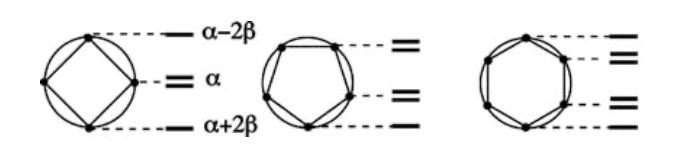
\includegraphics[width=3in]{F_cyclic_energy.png}
    \caption{Graphical illustration of cyclic energy}
    \label{F:cyclic_energy}
\end{figure}
This is true for cyclic groups $C_n$ if we check their character tables, as shown for group $C_4$, $C_5$ and 
$C_6$ in figure \ref{F_cyclic_group_table}

\begin{figure}[h!]
    \centering
    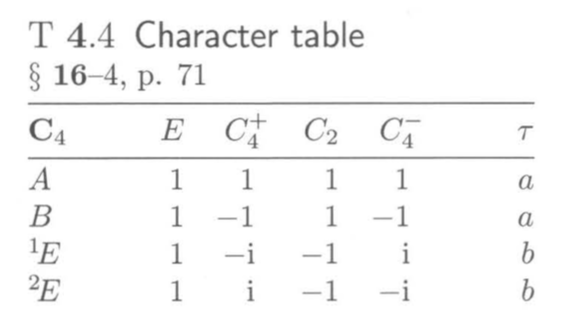
\includegraphics[width=3in]{F_C4.png}
    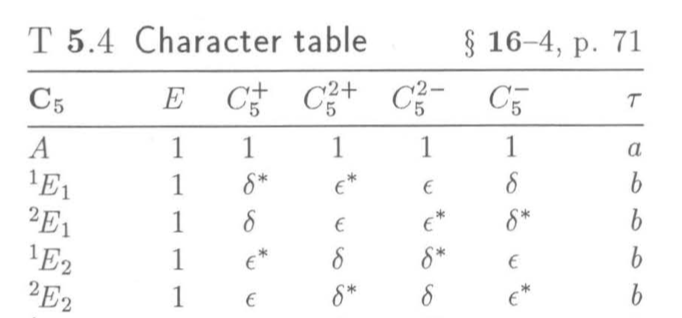
\includegraphics[width=3in]{F_C5.png}
    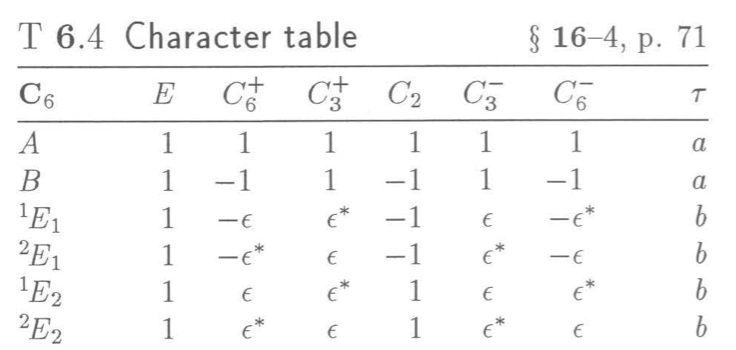
\includegraphics[width=3in]{F_C6.png}
    \caption{Character tables for cyclic groups}
    \label{F_cyclic_group_table}
\end{figure}

\subsection{Solids}


\end{document}
